
\documentclass{beamer}
\usepackage{bm}
\usetheme{Madrid}
\title{The BFGS Optimization Algorithm}
\author{Pratham Lalwani}
\institute{UC Merced}
\date{\today}
\usepackage{algorithm}
\usepackage{algorithmic}
\newcommand{\incfig}[1]{%
		\def\svgwidth{\columnwidth}
		\import{./figs/}{#1.png}
	}
\begin{document}

\frame{\titlepage}

\begin{frame}{Outline}
	\tableofcontents
\end{frame}

%------------------------------------------------
\section{Background}
\begin{frame}{Problem Setup}
	\begin{itemize}
		\item Given $f:\mathbb{R}^n \to \mathbb{R}$, say we are interested is minimizing the function, which is,
		      \[
			      \min_{\bm x\in \mathbb{R}^n} f(\bm x)
			      .\]
		\item From calculus, $\nabla f(\bm x) = \bm 0$ and solve analytically if it can be done.
		\item This problem arises everywhere especially nowadays with Machine Learning where $f(\bm x)$ is usually a cost function we are trying to minimize.
	\end{itemize}
\end{frame}

\begin{frame}{Gradient Descent and Its Limitations}
	\begin{itemize}
		\item With no way to compute a analytic solution one might turn a simple algorithm like Gradient Descent. \pause
		\item The next iterate is given by : $\bm x_{k+1} = \bm x_k - \gamma \nabla f(\bm x_k)$, where $\gamma$ is a fixed constant called step size or learning rate. \pause
		\item Pros: simple, easy to implement and not computationally expensive (per step) \pause
		\item Cons: slow convergence, sensitivity to step size.\pause
	\end{itemize}
\end{frame}
\begin{frame}[t]
	\frametitle{Gradient Descent}
	\begin{figure}[htpb]
		\centering
		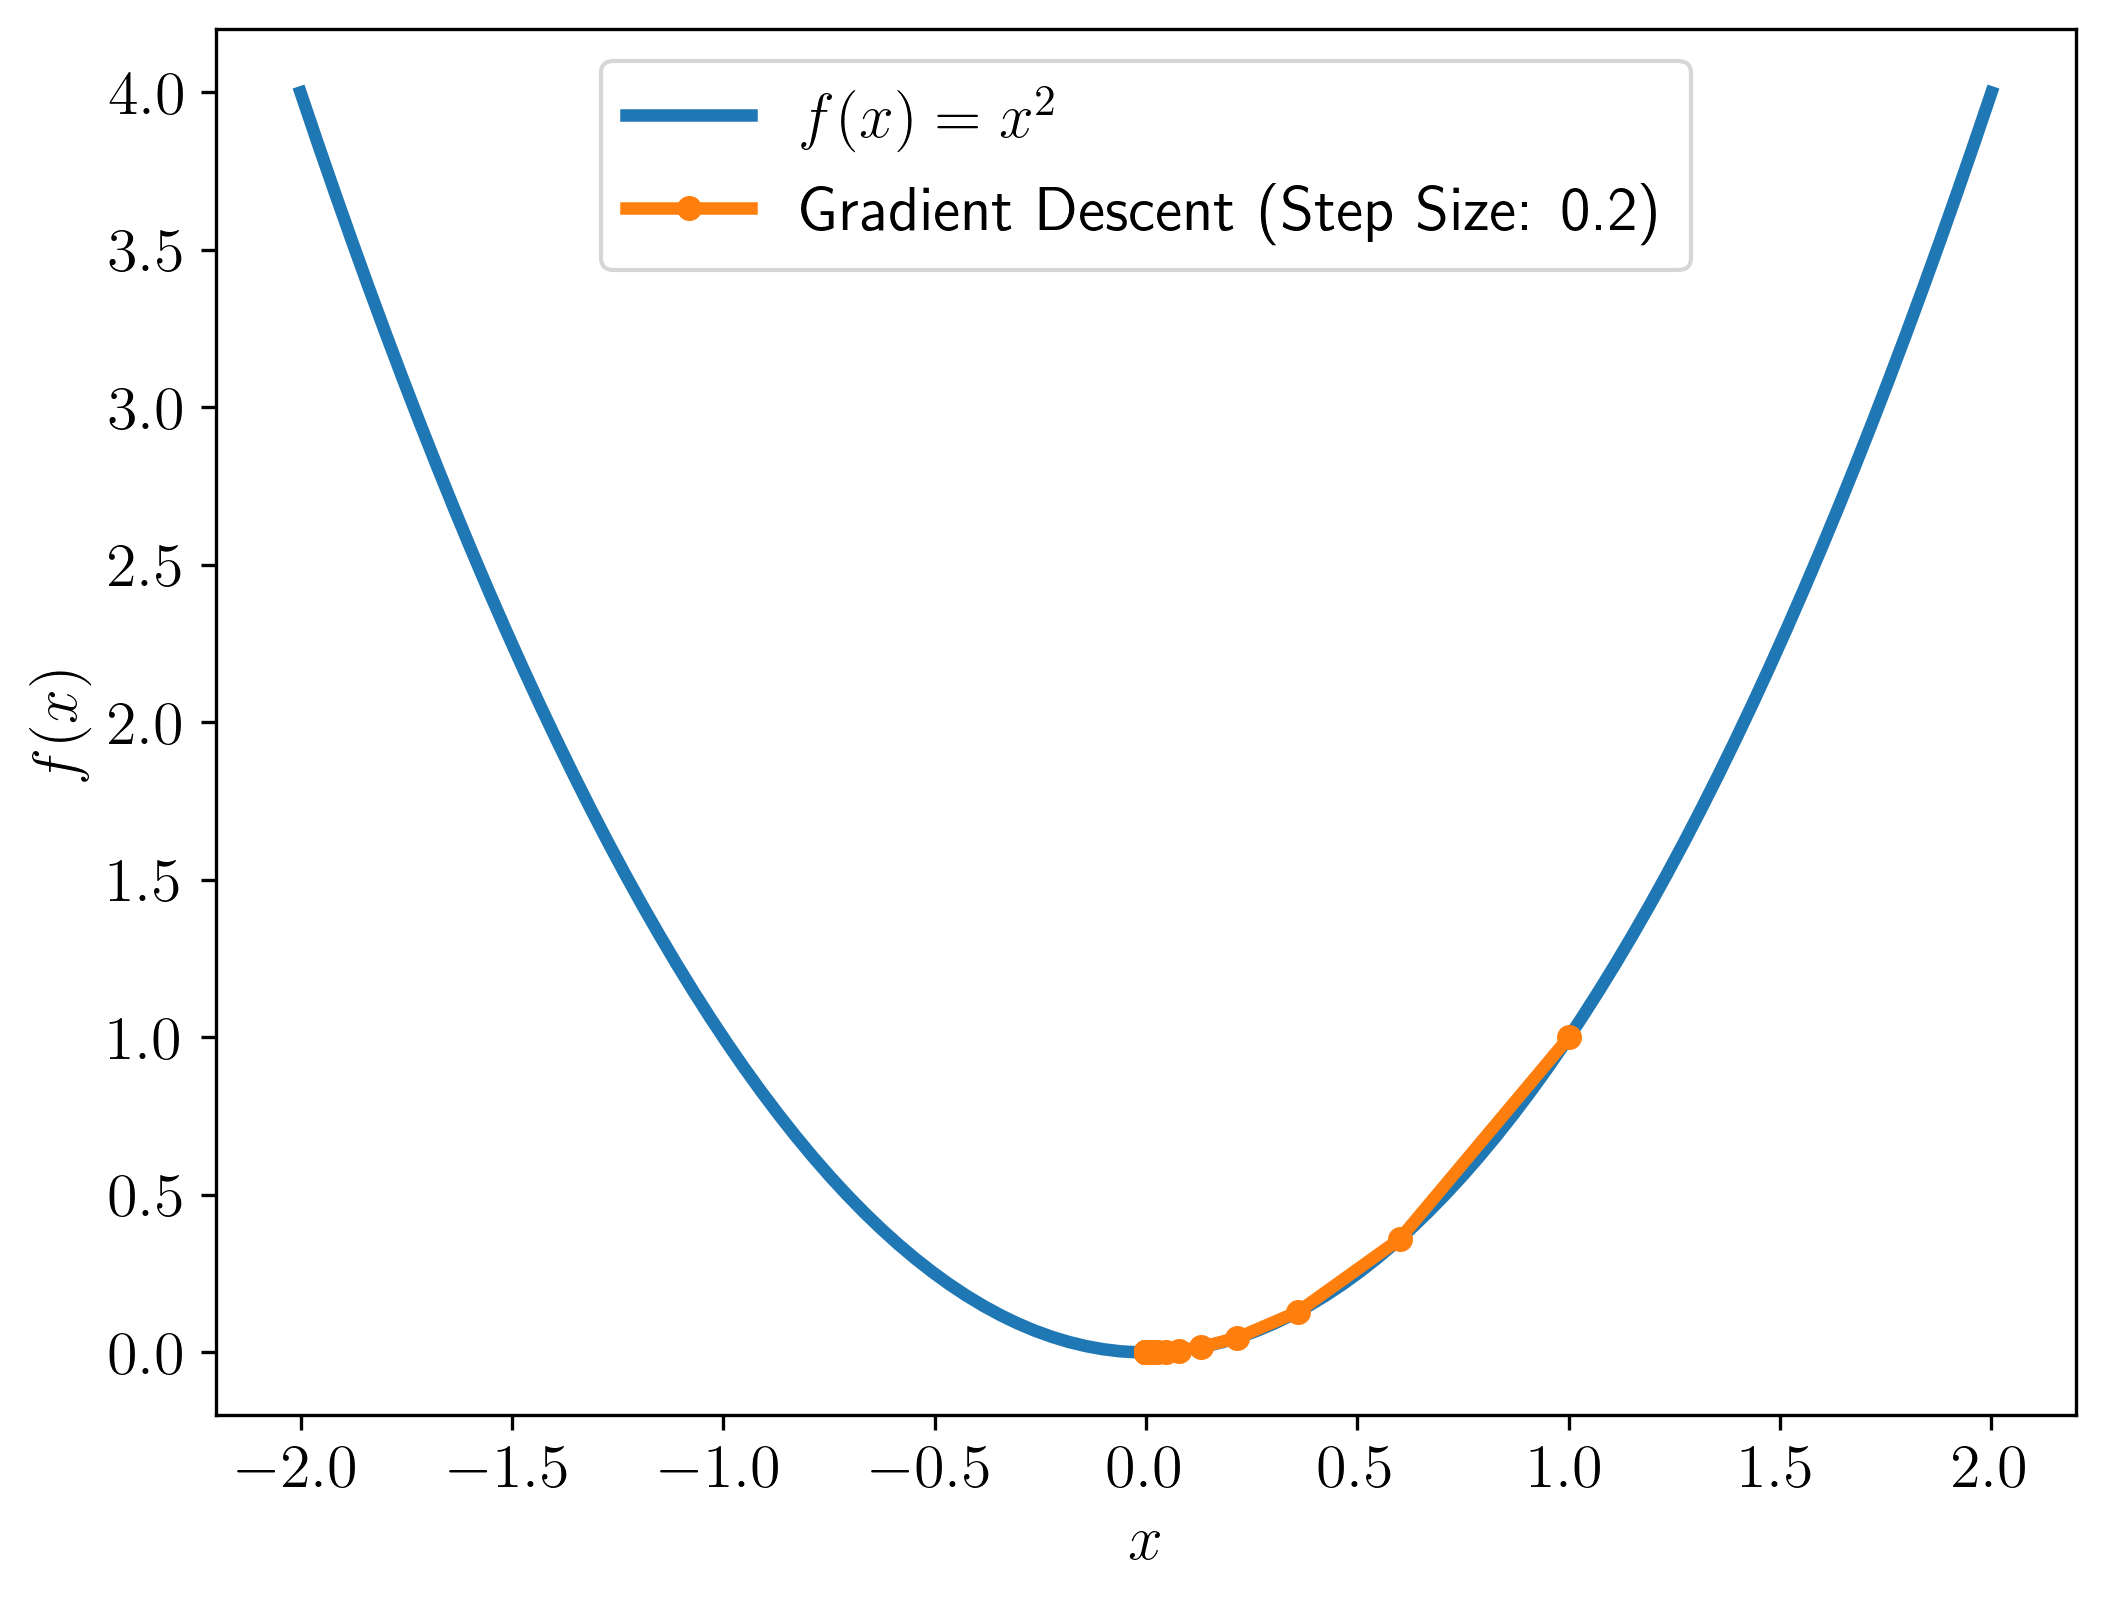
\includegraphics[width=0.7\textwidth]{./figs/gradient_descent_low_learning_rate}
		\caption{Gradient Descent on $x^2$}
		\label{fig:}
	\end{figure}
\end{frame}
\begin{frame}[t]
	\frametitle{Gradient Descent}
	\begin{figure}[htpb]
		\centering
		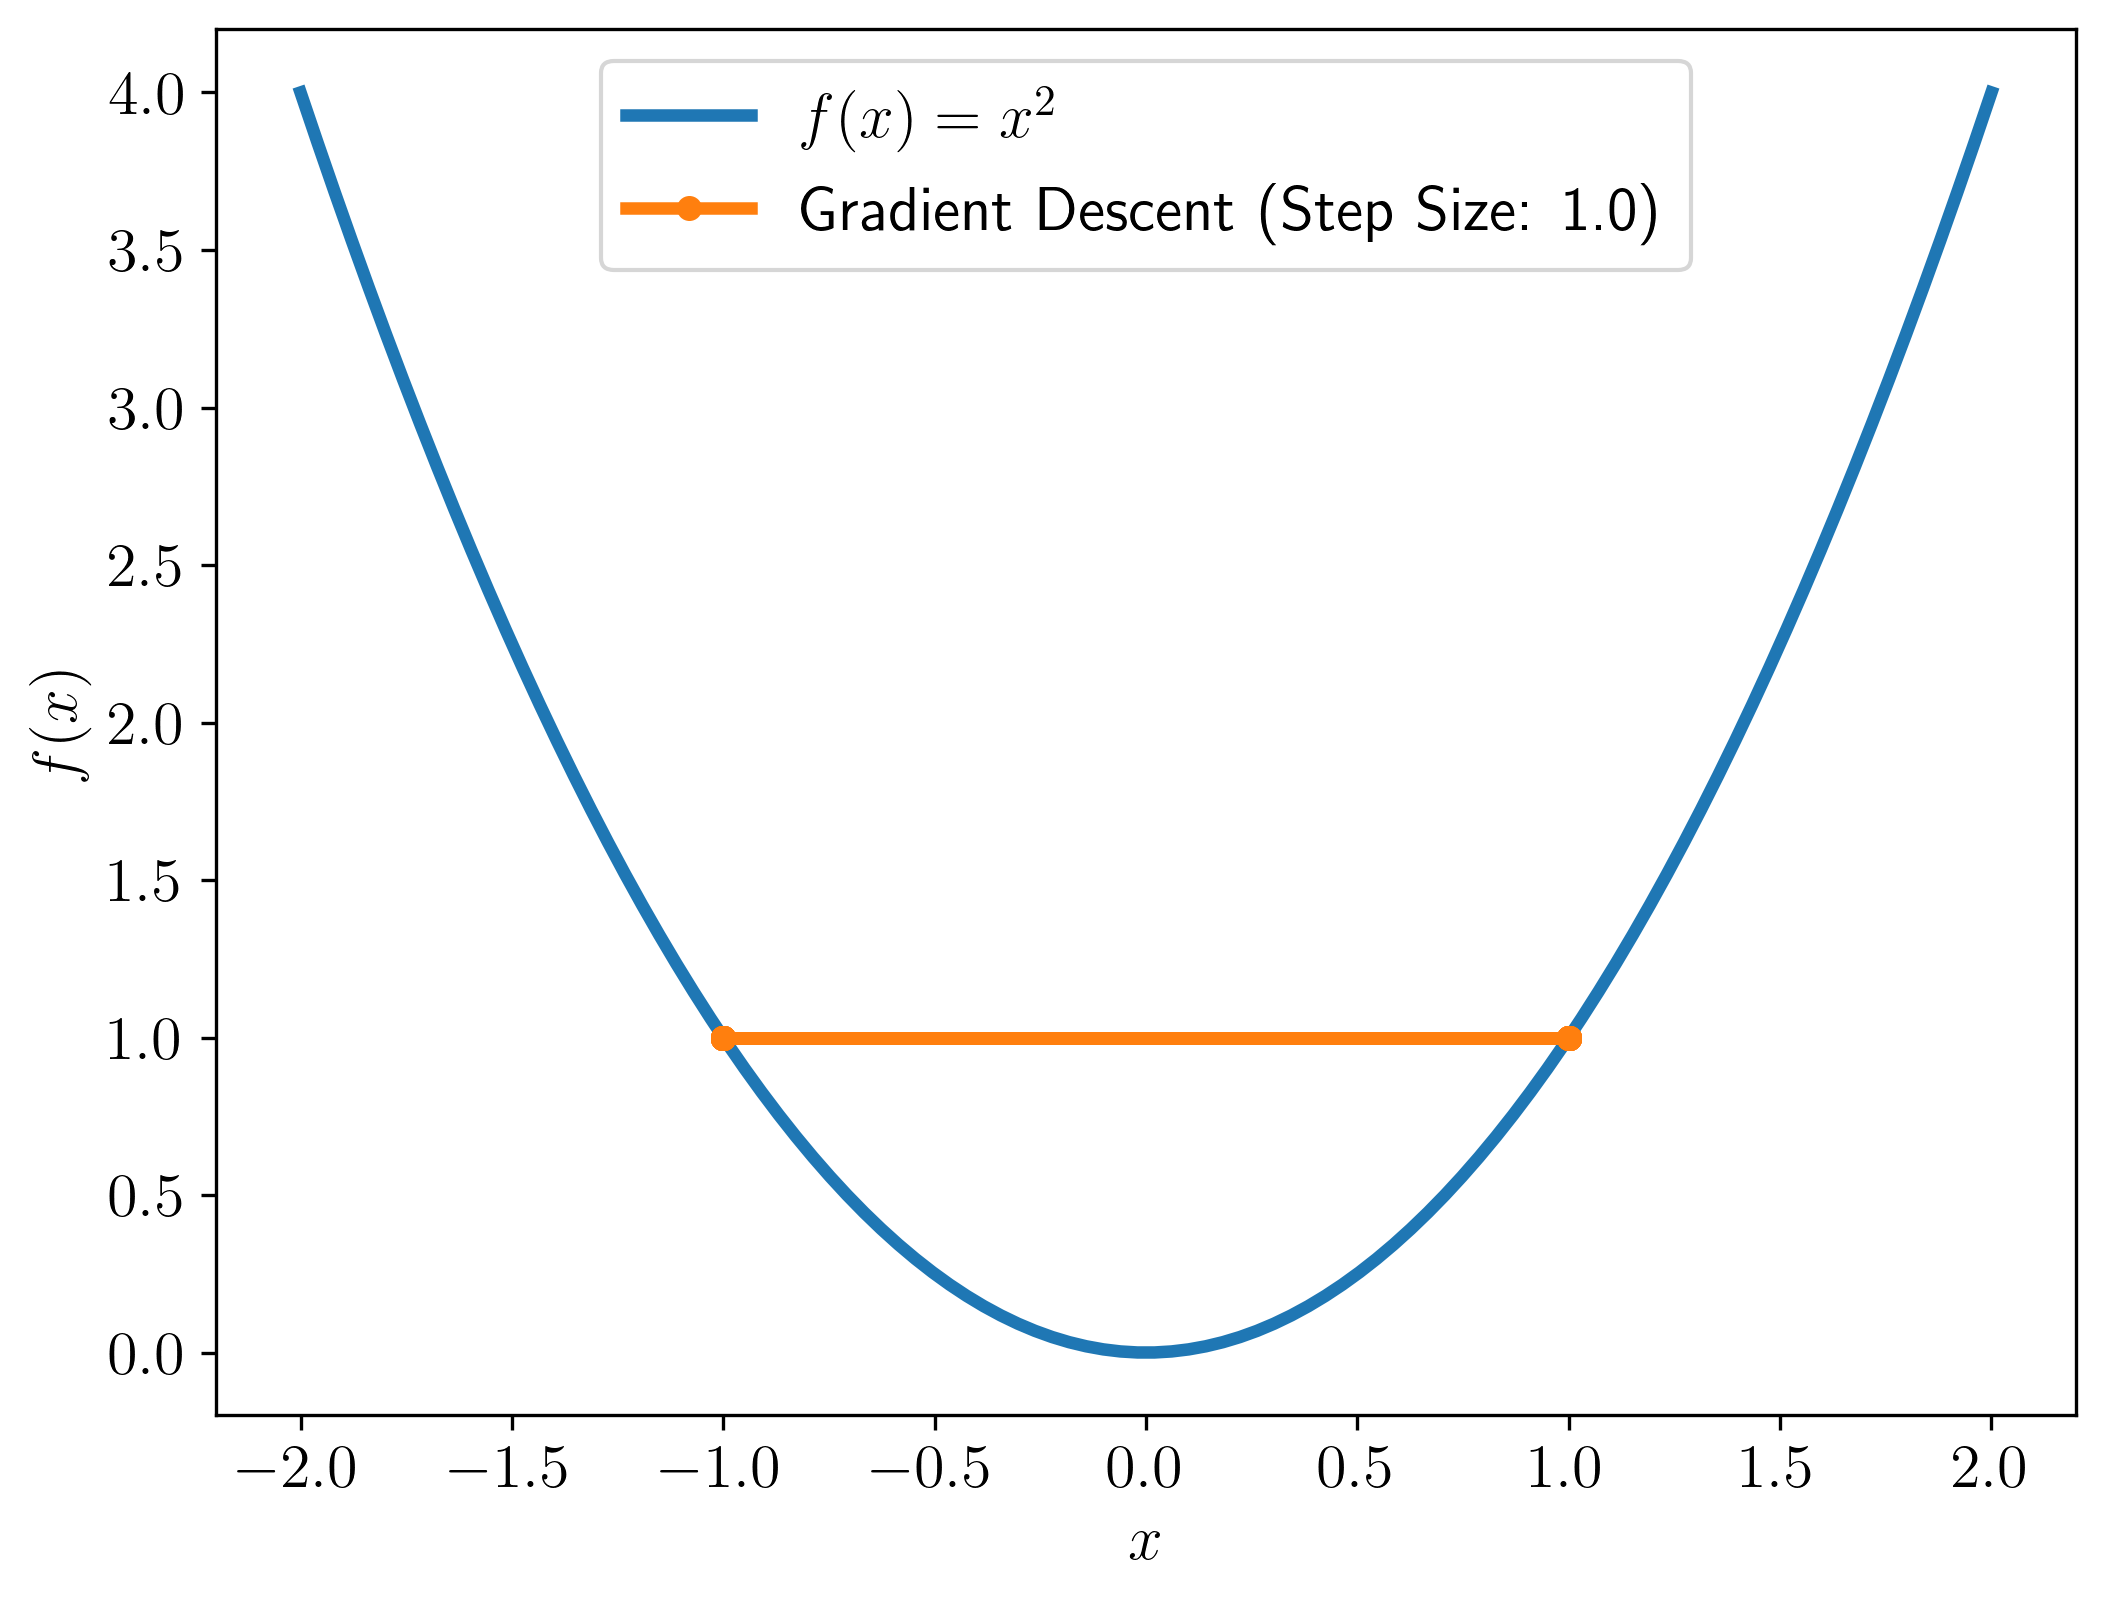
\includegraphics[width=0.7\textwidth]{./figs/gradient_descent_high_learning_rate}
		\caption{Gradient Descent on $x^2$}
		\label{fig:}
	\end{figure}
\end{frame}
%------------------------------------------------
\begin{frame}[t]
	\frametitle{But wait a minute}
	Instead of having a fixed Learning Rate what if we have a adaptive learning rate, which is "greedy".
	If we have,
	\[
		\bm x_{k+1} = \bm x_{k} - \alpha_k \nabla f(\bm x)
		.\]\pause
	We define,
	\[
		\phi(\alpha) := f(\bm x_k-\alpha \nabla f(\bm x))
		.\]\pause
	Now we solve the problem,
	\[
		\min_{\alpha \in [0,1]} \phi(\alpha)
		.\]\pause
	The good this about this problem is that it is one-dimensional. But we still have to realize the function we are evaluating underneath might be expensive to evaluate.
\end{frame}
\begin{frame}[t]
	\frametitle{Line Search}
	Now there are tons of techniques to find the minimum of a 1-D function. We shall use the one which is most familiar to us which is bisection method. \pause
	But, when should we terminate?\\\pause
	There is 2 conditions usually that we need to follow,\\
	Sufficient Decrease:
	\[
		f(\bm x- \alpha_k \nabla f(\bm x_k)  \le f(x_k) + c_1 \alpha_k \|\nabla f\|^2
		.\]
	and curvature condition,
	$$
		\nabla f\left(x_k+\alpha_k p_k\right)^T p_k \geq c_2 \nabla f_k^T p_k
	$$
	These two together make the Wolfe conditions of sufficient decrease.
\end{frame}
\begin{frame}[t]
	\frametitle{A picture is worth thousand words}
	\begin{figure}[htpb]
		\centering
		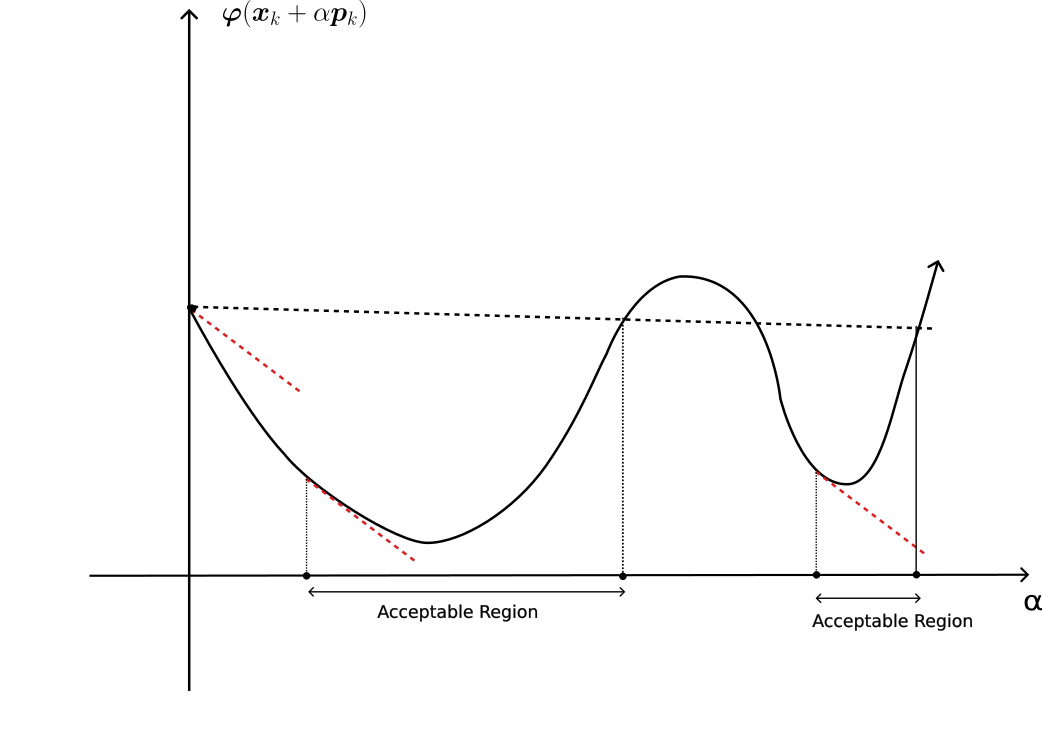
\includegraphics[width=0.7\textwidth]{drawing.png}
		\caption{Strong Wolfe Condition acceptance regions}
		\label{fig:3}
	\end{figure}

\end{frame}
\begin{frame}[t]
	\frametitle{Steepest Descent \& Newton}
	\begin{itemize}
		\item As we know steepest descent has it's own problems such as "zig-zag" behaviour as discussed in class. Thus we would like a better method.
		\item We also learnt about Newton Update for minimizing scalar functions which is given by
		      \[
			      \bm x_{k+1} = \bm x_k - H_f(\bm x_k)^{-1}\nabla f(\bm x_k)
			      .\]
		      Where $H_f$ is the hessian of  $f$ w.r.t  $\bm x$
		\item This is computationally quite expensive as it requires solving a linear system which takes $\mathcal O (n^3)$ time to solve. Where $n$ is problem dimension.
	\end{itemize}

\end{frame}
%------------------------------------------------
\section{Quasi-Newton Methods}
\begin{frame}{Quasi-Newton}
	\begin{itemize}
		\item We would like to develop a Hessian which doesn't take $O(n^3)$ time to solve.
		\item Before we do that some notation. All the algorithms we saw before now take the form
		      \[
			      \bm x_{k+1} = \bm x_k + \alpha_k \bm p_k
			      .\]
		      Where $\bm p_k$ is a descent direction.
		      We define $y_k = \nabla f(\bm x_{k+1}) - \nabla f(\bm x_{k})$ and $s_{k} = x_{k+1}- x_{k}$.
		      We would like to mimic the Newton search direction, which is
		      $\bm p_k^{Newton} = -H_f(x_k)^{-1}\nabla f(\bm x)$.
		      We would like a approximate hessian $ B_k \approx H_f(x_k)$ which doesn't take $\mathcal{O}(n^2)$ to compute.
			  \item These lead us to the BFGS update, introduced by Broyden, Fletcher, Goldfarb and Shanno over the course of 4 papers.
	\end{itemize}
\end{frame}
\begin{frame}[t]
	\frametitle{BFGS Derivation Outline}
	We start by defining a convex quadratic model as at step $k$ as:
	\[
		m_{k}(p) = f(\bm x_k) + \nabla f(\bm x_{k})^\top + \frac{1}{2} \bm p^\top B_k \bm p
		.\]
	The unique minimizer of this quadratic is
	\[
		p_{k} = -B_k^{-1} \nabla f(\bm x_k)
		.\]
	Now instead of recomputing $B_{k+1}$ for next iteration we proceed as follows,\\
	We would like to have $\nabla m_{k+1}(\bm 0) = \nabla f(\bm x_k)$ and $\nabla m_{k+1}(\bm -\alpha_k \bm p_k) = \nabla f(\bm x_k)$ to provide a good approximation to the objective function $f$ around those points.\\
	The first one we get for free,
	\[
		\nabla m_{k+1}(\bm 0) = \nabla f(\bm x_k)
		.\]
	The second one simplifies to,
	\[
		B_{k+1} s_k=y_k
		.\]
	This is the secant equation for the second derivative.
\end{frame}
\begin{frame}[t]
	\frametitle{BFGS Derivation Outline}
	The key benefit of BFGS is that it computes the inverse Hessian directly.\\
	Which means we directly find $H_{k+1}$ such that,
	\[
		B_{k+1}s_k = y_k \implies H_{k}y_k = s_k
		.\]
	We also would like to make the minimal update on $H_k$ to get $H_{k+1}$ and as mentioned earlier it is positive definite, \\
	Which results in the following constrained optimization problem,
	\[
		\min_{H\in \mathbb{R}^{n\times n}} \|W^{1/2}(H-H_k)W^{1/2}\|_F \qquad \text{subject to } \: H=H^T \ \text{ and } Hy_k = s_k
		.\]
	Which gives the formula:
	$H_{k+1}=\left(I-\rho_k s_k y_k^T\right) H_k\left(I-\rho_k y_k s_k^T\right)+\rho_k s_k s_k^T$
	Which is the BFGS update.\\
	Great thing about it is that it is a small rank-2 update and still keeps the matrix positive definite.
\end{frame}
%------------------------------------------------
\begin{frame}[t]
	\frametitle{Algorithm 6.1 (BFGS Algorithm)}
	\begin{algorithm}[H]
		\caption{(BFGS Algorithm)}
		\label{alg:bfgs}
		\begin{algorithmic}[1]
			\REQUIRE Given starting point $x_0$, convergence tolerance $\epsilon > 0$, inverse Hessian approximation $H_0$;
			\STATE $k \leftarrow 0$;
			\WHILE{$\| \nabla f_k \| > \epsilon \quad \& \quad k<\text{maxIter}$}
			\STATE Compute search direction
			\STATE $p_k = -H_k \nabla f_k$;
			\STATE Set $x_{k+1} = x_k + \alpha_k p_k$ where $\alpha_k$ is computed from a line search procedure to satisfy the Wolfe conditions;
			\STATE Define $s_k = x_{k+1} - x_k$ and $y_k = \nabla f_{k+1} - \nabla f_k$;
			\STATE Compute $H_{k+1}$ ;
			\STATE $k \leftarrow k + 1$;
			\ENDWHILE
		\end{algorithmic}
	\end{algorithm}
\end{frame}
%------------------------------------------------
\section{Rosenbrock Example}
\begin{frame}{Rosenbrock Example}
	\begin{itemize}
		\item Test function: $f(x,y) = (a - x)^2 + b(y - x^2)^2$
		\item Typical parameters: $a=1, b=100$
		\item Illustrates curved valley and optimization challenge
	\end{itemize}
\end{frame}

\begin{frame}{Rosenbrock Example Results}
	\begin{figure}
		\centering
		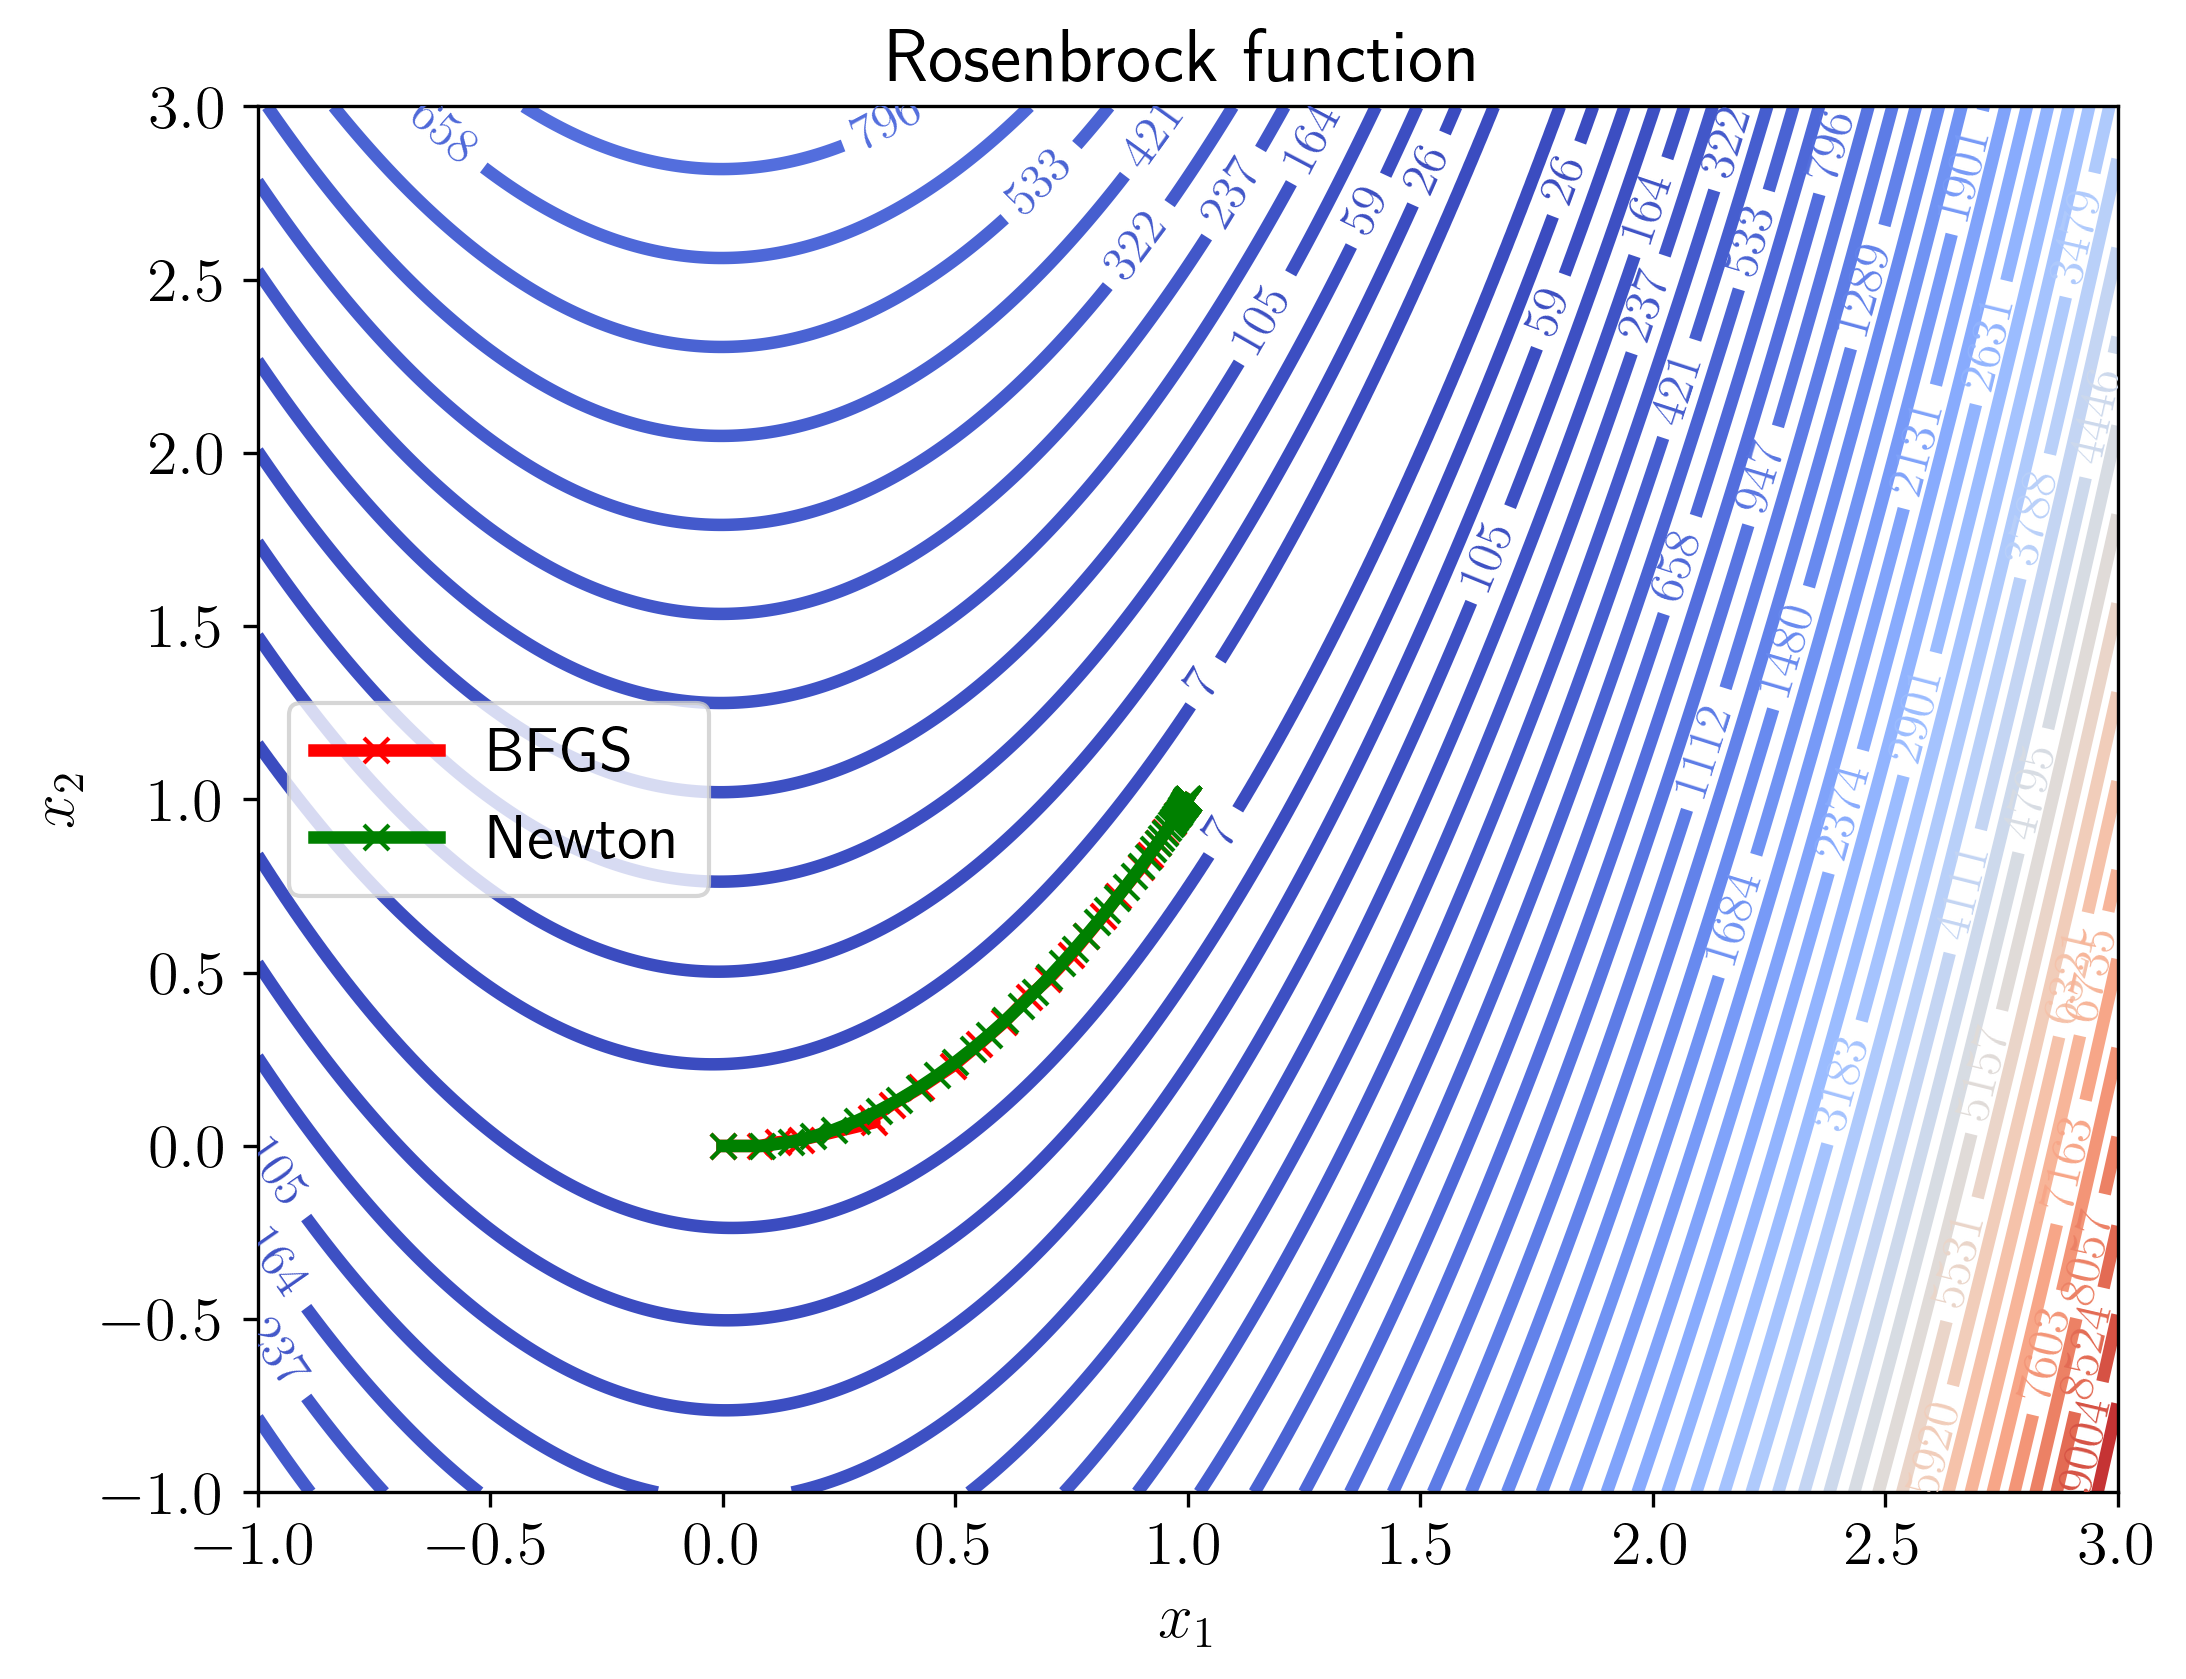
\includegraphics[width=0.6\textwidth]{./figs/rosenbrock_contour.png}
		\caption{BFGS optimization path on Rosenbrock function}
	\end{figure}
\end{frame}

\begin{frame}{Rosenbrock Example Results}
	\begin{figure}
		\centering
		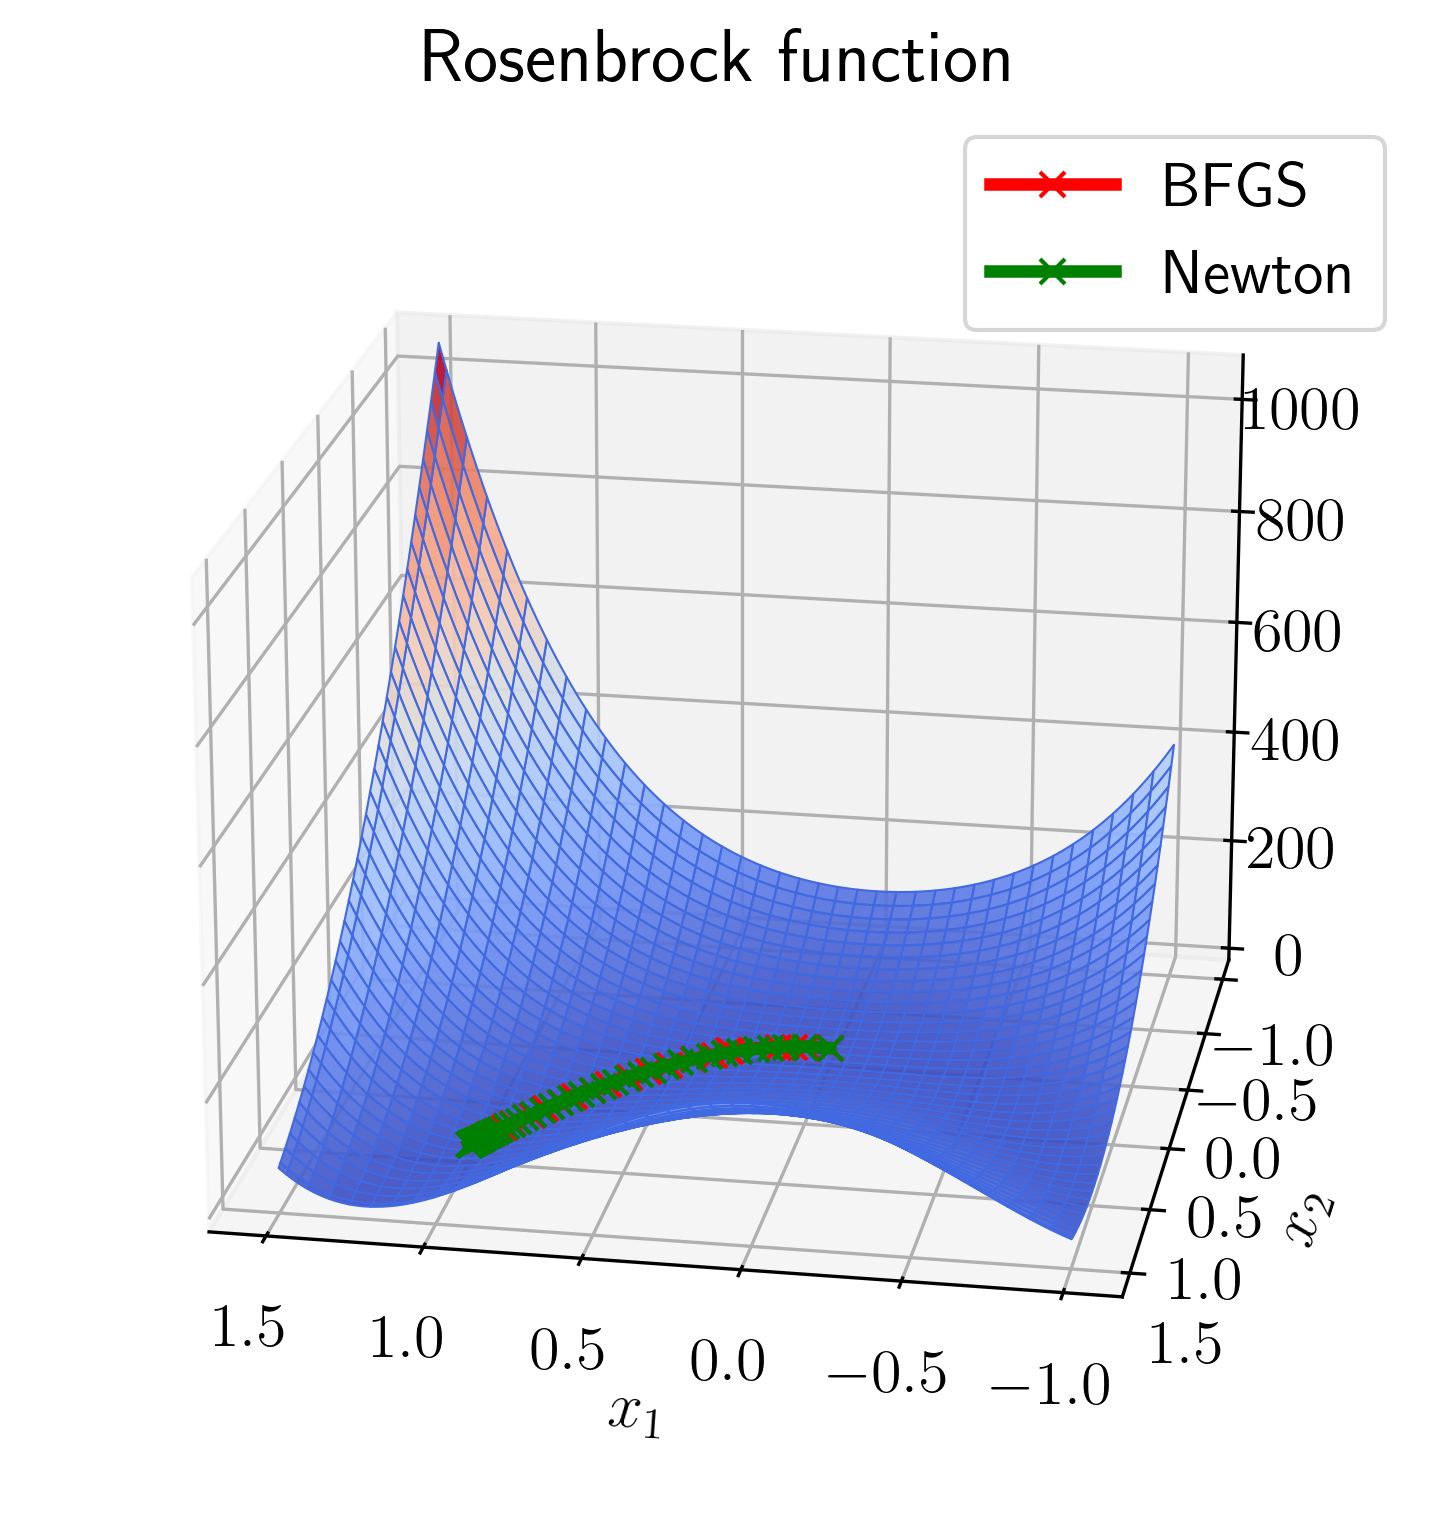
\includegraphics[width=0.6\textwidth]{./figs/rosenbrock_surface.png}
		\caption{BFGS optimization path on Rosenbrock function}
	\end{figure}
\end{frame}
%------------------------------------------------
\section{Results}
\begin{frame}{Results}
	\frametitle{Results}
	\tabcolsep=0.11cm
	\begin{tabular}{|l|l|l|l|l|}
		\hline
		Function                       & BFGS     & Newton   & LBFGS    & GD       \\
		\hline
		Adjiman Function (2-D)         & nan      & 4.61e-05 & 5.50e-16 & 7.70e-01 \\
		\hline
		Rosenbrock N-D (100-D)         & 9.28e-11 & 5.13e-04 & 9.24e-11 & 2.92e+00 \\
		\hline
		Paviani Function (10-D)        & nan      & nan      & nan      & 8.72e-02 \\
		\hline
		Csendes Function (10-D)        & 9.57e-11 & 1.21e-03 & 9.16e-11 & 7.48e-02 \\
		\hline
		Griewank Function (2-D)        & nan      & 1.26e-15 & 6.65e-11 & 8.31e-09 \\
		\hline
		Hosaki Function (2-D)          & nan      & 3.17e-05 & nan      & 8.66e-02 \\
		\hline
		Brent Function (2-D)           & 9.00e-11 & 2.51e-05 & 9.90e-11 & 3.67e+00 \\
		\hline
		Giunta Function (2-D)          & 2.22e-15 & 9.40e-05 & 2.67e-15 & 1.29e-08 \\
		\hline
		Styblinski-Tang Function (2-D) & 2.93e-14 & 1.12e-04 & 6.39e-14 & 9.96e-11 \\
		\hline
		Trid 6 Function (6-D)          & nan      & 2.47e-05 & nan      & 4.08e+00 \\
		\hline
		\hline
	\end{tabular}

\end{frame}

%------------------------------------------------

%------------------------------------------------
\section{Conclusion}
\begin{frame}{Conclusion}
	\begin{itemize}
		\item Introduced BFGS as an quasi Newton optimzer.
		\item Provided description of Wolfe conditions, and an outline of BFGS derivation.
		\item Compared BFGS against other methods.
	\end{itemize}
\end{frame}

\end{document}

